\section{Solution to the basic environment: \textit{move0}}
In this section, we compare the proposed W-KTR method with other state-of-art algorithms on the basic \textit{move0} environment.

The performance of W-KTR algorithm is shown in Figure \ref{rec_move0_wktr_tune}:

\begin{figure}[h]
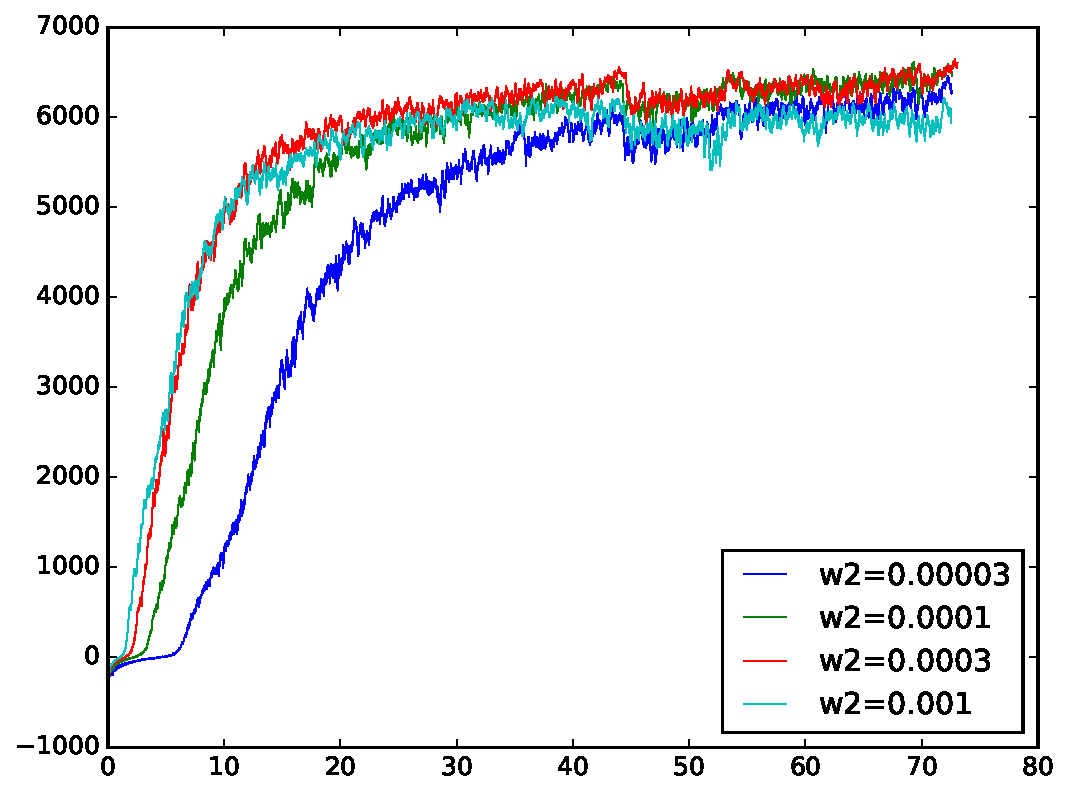
\includegraphics[width=\textwidth]{images/rec_move0_wktr_tune.pdf}
\centering
\caption{Performance of move0 W-KTR agent with diferent hyper-parameter $\delta_W^2$, the x-axis is the number of million timesteps and the y-axis is the total episode reward averaged over the last 200 episodes}
\end{figure}\label{rec_move0_wktr_tune}
It can be shown that the W-KTR agent has a stable final performance, which is not much dependent on the hyper-parameter $\delta_W^2$.

The performance of ACKTR agents is shown in Figure \ref{rec_move0_acktr_tune}:
\begin{figure}[h]
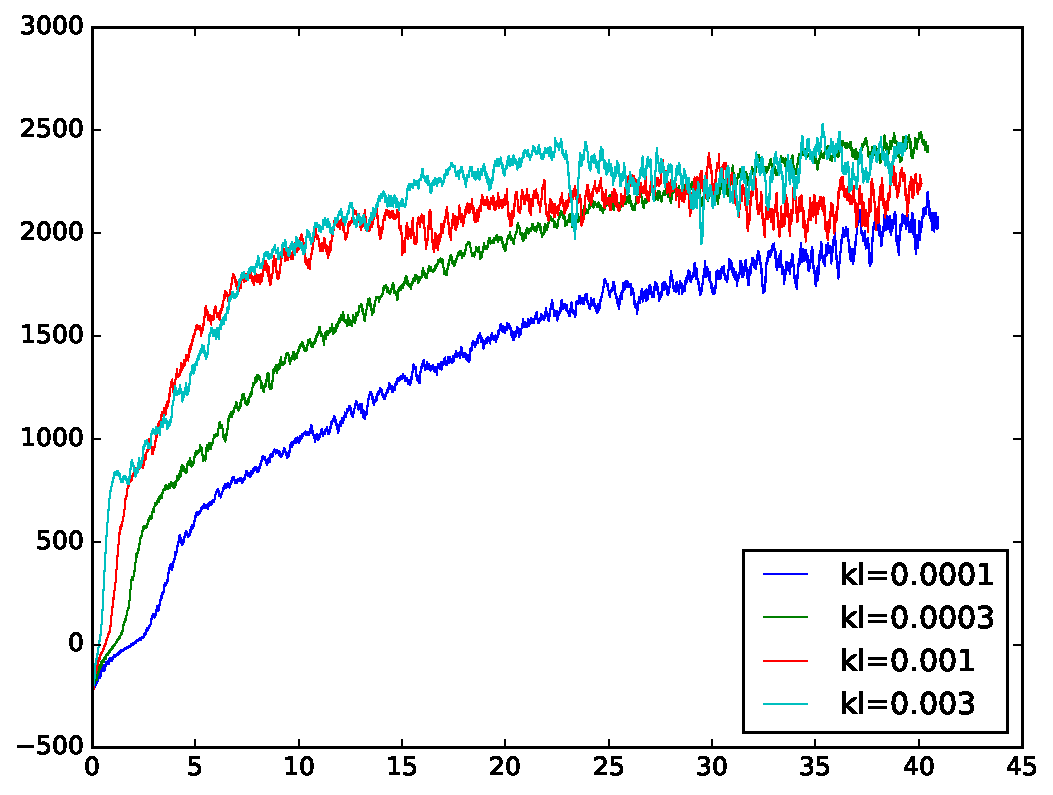
\includegraphics[width=\textwidth]{images/rec_move0_acktr_tune.pdf}
\centering
\caption{Performance of move0 PPO agent with diferent hyper-parameter $\delta_{kl}$, the x-axis is the number of million timesteps and the y-axis is the total episode reward averaged over the last 200 episodes}
\end{figure}\label{rec_move0_acktr_tune}
It can be shown that the ACKTR agent can achieve a faster rate of improvement at the first 10 million steps, but the improvement rate becomes slow as the training proceeds. The agents tend to stuck at sub-optimal policies since the policies converge too fast and cannot effectively adjust once the STD becomes small.

We also run experiments on tuning a PPO agent for the task move0, which is shown in Figre~\ref{rec_move0_ppo_tuning}. The original PPO algorithms has 40 minibatch updates in each batch, which converges too early. We only performa one gradient update over the whole batch in this experiment. The performance of the PPO agent appears to be sensitive to the hyper-parameter, and the agent can't avoid the drop of performance in the late phase of training. The method also needs to trade-off between the early improvement rate and the final performance. In conclusion, the PPO method is not a robust algorithm.
\begin{figure}[h]
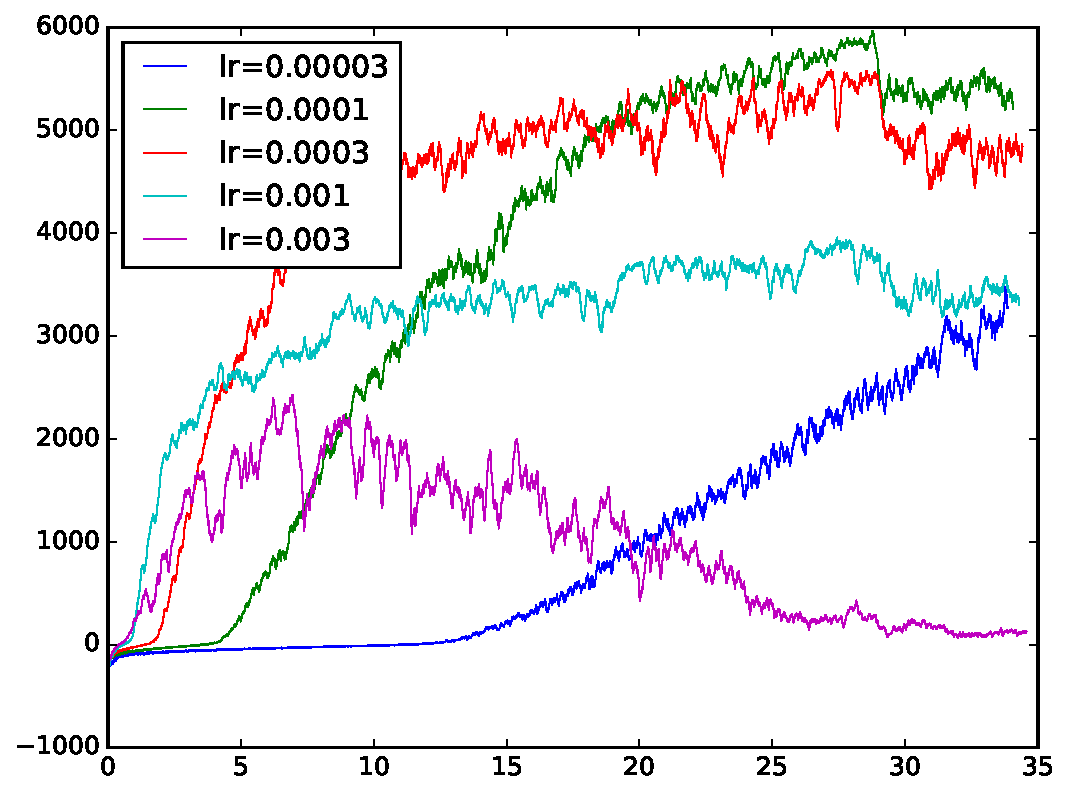
\includegraphics[width=\textwidth]{images/rec_move0_ppo_tuning.pdf}
\centering
\caption{Performance of move0 PPO agent with diferent hyper-parameter $learning rate$, the x-axis is the number of million timesteps and the y-axis is the total episode reward averaged over the last 200 episodes}
\end{figure}\label{rec_move0_ppo_tuning}

All the method above use a batch size of 4000 timesteps produced by 20 parallel agents.

\section{Flat solution to a simple Multi-Modality environment: \textit{move1d}}
In the move1d environment, the agent needs to learn from the image input to decide whether to move forward or backward, as well as control according to the states.
We have tried to solve the problem using ACKTR method, presented in Figure~\ref{rec_flatmove1d_acktr_tune}, shows that the agent can easily get stuck at the score of 1000, and cannot improve much even if the agent breaks the bottleneck because the average STD parameter already drops to below 0.04.
\begin{figure}[h]
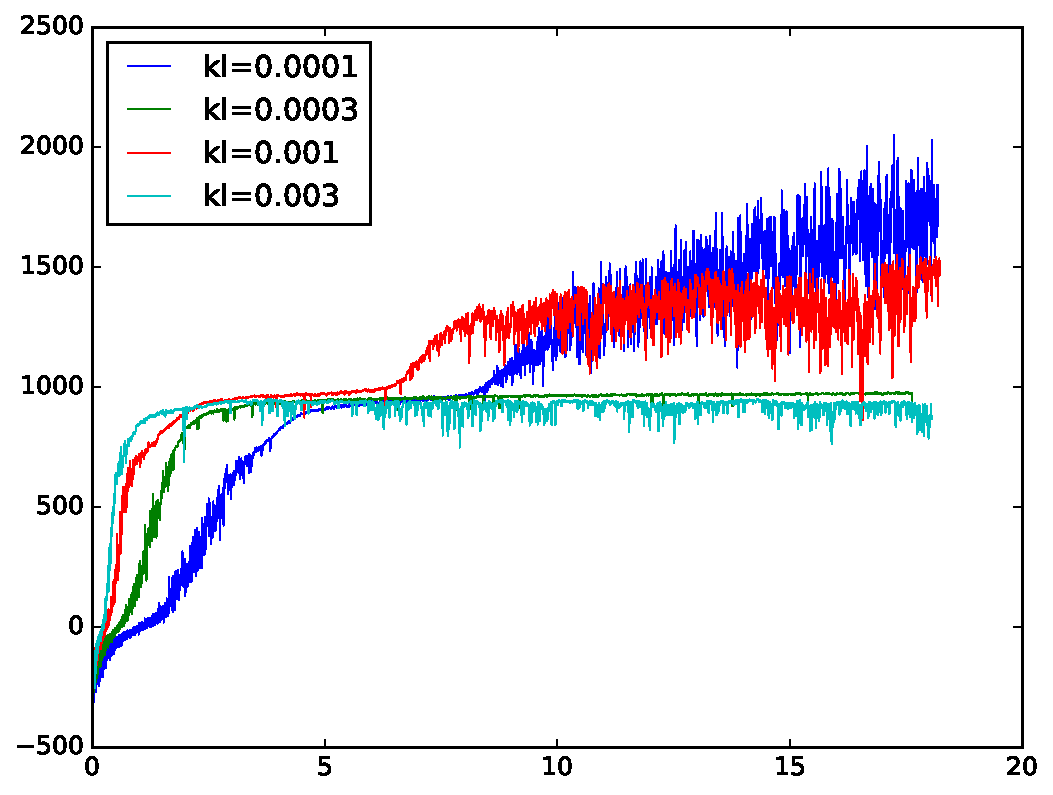
\includegraphics[width=\textwidth]{images/rec_flatmove1d_acktr_tune.pdf}
\centering
\caption{Performance of move1d ACKTR agent with diferent hyper-parameter $learning rate$, the x-axis is the number of million timesteps and the y-axis is the total episode reward averaged over the last 20 episodes}
\end{figure}\label{rec_flatmove1d_acktr_tune}

We also did a single experiment using the proposed W-KTR method, and is shown in Figure~\ref{rec_flatmove1d_wktr}. The W-KTR agent manages to achieve a fast improvement rate and high final performance after getting stuck at the bottleneck score 1000 for a while.
\begin{figure}[h]
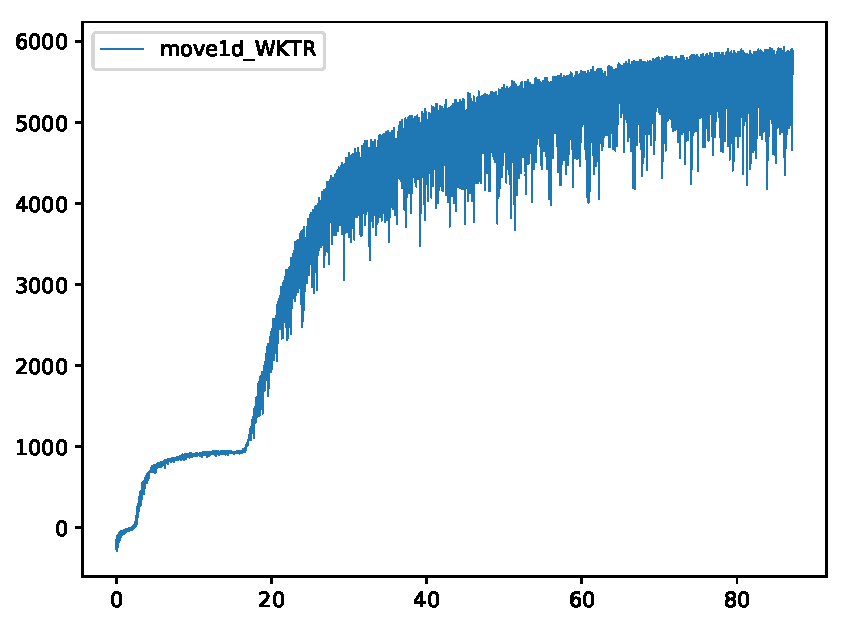
\includegraphics[width=\textwidth]{images/rec_flatmove1d_wktr.pdf}
\centering
\caption{Performance of move1d W-KTR agent with  hyper-parameter $\delta_W^2= 0.0001$, the x-axis is the number of million timesteps and the y-axis is the total episode reward averaged over the last 20 episodes}
\end{figure}\label{rec_flatmove1d_wktr}

This proves that the W-KTR agent is better at handle local minimum and re-adjust the agent's policy even when the policy STD becomes low.


